\documentclass[review,3p,times,12pt,letterpaper]{elsarticle}

\usepackage{amsmath}
\usepackage{amssymb}
\usepackage{booktabs}
\usepackage{graphicx}
\usepackage{lineno}
\usepackage{url}
\usepackage{xcolor}

\emergencystretch=3em
\Urlmuskip=0mu plus 1mu\relax

\linenumbers

\journal{Alzheimer's \& Dementia}

\begin{document}

\begin{frontmatter}

\title{Motor Network Impairment as a Potential Early Biomarker for Alzheimer's Disease}
%\title{Motor-system MRI correlates of amyloid PET burden in adults with preserved MMSE: an OASIS-3 study}


\author[inst1]{Anand A. Joshi\corref{cor1}}
\author[inst3]{Ronald Salloum}
\author[inst1]{Richard M. Leahy}
\author[inst2]{Daniel J. Tward}
\author[inst2]{David W. Shattuck}
\author[inst4]{Abhijit J. Chaudhari}

\cortext[cor1]{Corresponding author: Anand A. Joshi. Postal address: Ming Hsieh Department of Electrical and Computer Engineering, 3740 McClintock Avenue, EEB 426, Los Angeles, CA, 90089-2560, USA. Email: \texttt{ajoshi@usc.edu}}

\affiliation[inst1]{organization={University of Southern California}, city={Los Angeles}, postcode={90089}, state={CA}, country={USA}}
\affiliation[inst2]{organization={University of California Los Angeles}, city={Los Angeles}, postcode={90095}, state={CA}, country={USA}}
\affiliation[inst3]{organization={California State University, San Bernardino}, city={San Bernardino}, postcode={92407}, state={CA}, country={USA}}
\affiliation[inst4]{organization={University of California Davis}, city={Davis}, postcode={95616}, state={CA}, country={USA}}

\begin{abstract}
\textbf{INTRODUCTION:} Motor dysfunction is increasingly recognized across the Alzheimer's disease (AD) spectrum. The objective of this study is to use neuroimaging data to investigate motor network impairment as a potential early biomarker for Alzheimer's disease.
\textbf{METHODS:} We analyzed OASIS-3 participants with Mini-Mental State Examination (MMSE) scores $>24$. Their amyloid positivity was defined using tracer-specific partial-volume-corrected mean cortical SUVR cutoffs from OASIS-3: PiB $>1.42$ and AV45 $>1.19$. We tested whether PET amyloid burden was associated with cortical thickness and whether PET-defined amyloid status was associated with resting-state fMRI motor-network connectivity alterations. In addition, we performed an MMSE-based fMRI analysis as an exploratory analysis of the impact of early AD on motor networks.
\textbf{RESULTS:} The final cohort with available PET data
and preserved cognition ($\text{MMSE} > 24 $) 
included 485 participants (138 A+, 347 A-).  
A+= participants were older ($72.73 \pm 6.62$ vs. $65.91 \pm 8.67$ years, 
$p = 1.5 \times 10^{-18}$), differed in sex distribution ($p = 0.013$), and had slightly lower MMSE scores despite remaining above the inclusion threshold ($28.43 \pm 1.58$ vs. $29.05 \pm 1.15$, $p = 5.1 \times 10^{-5}$). In the subset used for surface-based statistics ($n = 398$), cortical thickness showed significant exploratory associations with amyloid PET SUVR in bilateral sensorimotor, cingulate, parietal, temporal, and insular regions. Differences in motor network connectivity between PET-defined groups were minimal. While the strongest uncorrected functional connection was between the left middle cingulate and inferior postcentral regions ($p = 0.002$), no connections survived multiple comparison correction (FDR $q = 0.091$), including in age- and sex-adjusted models (minimum FDR $q = 0.921$). Exploratory MMSE-based analyses revealed motor-region associations in Amplitude of low-frequency fluctuations (ALFF) and BrainSync pairwise regressions.
\textbf{DISCUSSION:} Amyloid burden is associated with cortical thickness reductions in sensorimotor regions in adults with globally preserved cognition, whereas resting-state functional connectivity alterations remain subtle. These findings suggest that motor-system structural phenotypes are relevant to early biological Alzheimer's disease pathways before overt clinical decline. Future longitudinal work incorporating tau biomarkers, direct motor phenotyping, and task-based fMRI is warranted to validate these structural associations and evaluate their clinical predictive value.
\end{abstract}

\begin{keyword}
Alzheimer's disease \sep amyloid PET \sep cortical thickness \sep motor cortex \sep resting-state fMRI \sep manual dexterity
\end{keyword}

\end{frontmatter}

\section{Background}

Alzheimer's disease (AD) is a major public health burden in older adults \cite{alzheimers_facts_2026}. Contemporary research frameworks and revised diagnostic criteria increasingly define AD biologically rather than solely by clinical symptoms \cite{sperling_toward_2011,dubois_preclinical_2016,jack_jr_niaaa_2018,jack_revised_2024}. Amyloid PET provides an in vivo biomarker of amyloid-$\beta$ pathology and can identify individuals on the AD biological spectrum before or near the onset of overt impairment. At the same time, amyloid positivity alone does not provide tau staging, autopsy confirmation, or proof that all observed neurodegeneration is AD-specific.

Motor dysfunction is documented in mild cognitive impairment (MCI) and AD and may predict later cognitive and functional decline \cite{camicioli_motor_1998,watson_executive_2010,wilson_parkinsonianlike_2003,buchman_grip_2007,scarmeas_motor_2005,koppelmans_neural_2022}. Fine motor functions, including finger tapping, gripping, and manual dexterity, require integration of primary motor, somatosensory, cingulate, parietal, and temporal systems \cite{smith_critical_1999,shinohara_effects_2003,frederiksen_age_2006,liou_hand_2020}. AD pathology has been reported in primary motor and supplementary motor areas \cite{arnold_topographical_1991,giannakopoulos_cerebral_1997,suva_primary_1999}, and recent biomarker studies link motor-cortex AD biomarker burden and regional tau burden to poorer dexterity or motor symptoms \cite{gupta_biomarker_dexterity_2024,na_neural_basis_2025}. These observations motivate neuroimaging studies of motor and sensorimotor systems in biomarker-characterized AD-spectrum cohorts.

Cognitive screening measures, including MMSE, do not by themselves establish AD pathophysiology. We therefore use amyloid PET status and amyloid PET burden from OASIS-3 as the primary biomarker variables. We ask whether motor-cortex structural and functional measures are altered in MMSE-preserved adults who are amyloid-positive by PET.

\section{Methods}

\subsection{Data source and participant selection}

We used OASIS-3, a longitudinal multimodal dataset of normal aging and AD that includes MRI, PET, dementia status, and clinical/cognitive measures \cite{lamontagne2019oasis}. OASIS-3 MRI data were acquired on Siemens 1.5T and 3T scanners, including a BioGraph mMR PET-MR 3T system. Six-minute eyes-open resting-state BOLD scans were available for functional analyses.

The primary cohort consisted of participants with MMSE $>24$ and an available amyloid PET measure matched to the MRI/PUP record. This produced 485 PET-linked participants with preserved global cognitive screening scores. Because MMSE $>24$ does not guarantee normal clinical status, we report Clinical Dementia Rating (CDR) closest to MRI and avoid treating this sample as uniformly cognitively normal. For cortical-thickness surface statistics we used the same image-quality subset as the available vertexwise analysis (n=398; 104 A+ and 294 A-). For PET-defined motor-connectivity analysis, 483 candidate participants had resting-state fMRI scans matched to PET and preserved MMSE; three candidate scans were excluded for non-finite ROI data, leaving 480 participants with usable time series (346 A- and 134 A+).

\subsection{Amyloid PET status}

OASIS-3 PET data were processed with the PET Unified Pipeline (PUP), which uses FreeSurfer regions, PET-to-MRI registration, and regional SUVR quantification \cite{oasis3_data_dictionary_2018,su_quantitative_2013}. We used the partial-volume-corrected mean cortical SUVR measure, \path{PET_fSUVR_rsf_TOT_CORTMEAN}. Amyloid positivity was defined by the OASIS-3 tracer-specific RSF mean cortical SUVR cutoffs: PiB $>1.42$ and AV45 $>1.19$ \cite{oasis3_data_dictionary_2018}. These cutoffs are consistent with Centiloid standardization efforts for amyloid PET quantification \cite{klunk_centiloid_2015}. The PET-linked cohort included 347 A- and 138 A+ participants (Table \ref{tab:cohort}). Amyloid-positive status was used as biomarker evidence of AD pathophysiology, not as a complete A/T/N staging diagnosis.

\begin{table}[t]
\centering
\caption{PET-linked MMSE-preserved cohort. Values are mean $\pm$ SD unless noted.}
\label{tab:cohort}
\begin{tabular}{lcc}
\toprule
Measure & A- & A+ \\
\midrule
N & 347 & 138 \\
Age, years & 65.91 $\pm$ 8.67 & 72.73 $\pm$ 6.62 \\
Female / male, n & 206 / 141 & 64 / 74 \\
PiB / AV45, n & 260 / 87 & 87 / 51 \\
CDR 0 / 0.5 / 1, n & 324 / 23 / 0 & 94 / 39 / 5 \\
MMSE closest to MRI & 29.05 $\pm$ 1.15 & 28.43 $\pm$ 1.58 \\
CDR closest to MRI & 0.03 $\pm$ 0.12 & 0.18 $\pm$ 0.28 \\
RSF mean cortical SUVR & 1.01 $\pm$ 0.13 & 2.25 $\pm$ 0.70 \\
Median PET-MRI gap, days & 17.0 & 31.5 \\
\bottomrule
\end{tabular}
\end{table}

\begin{figure}[t]
\centering
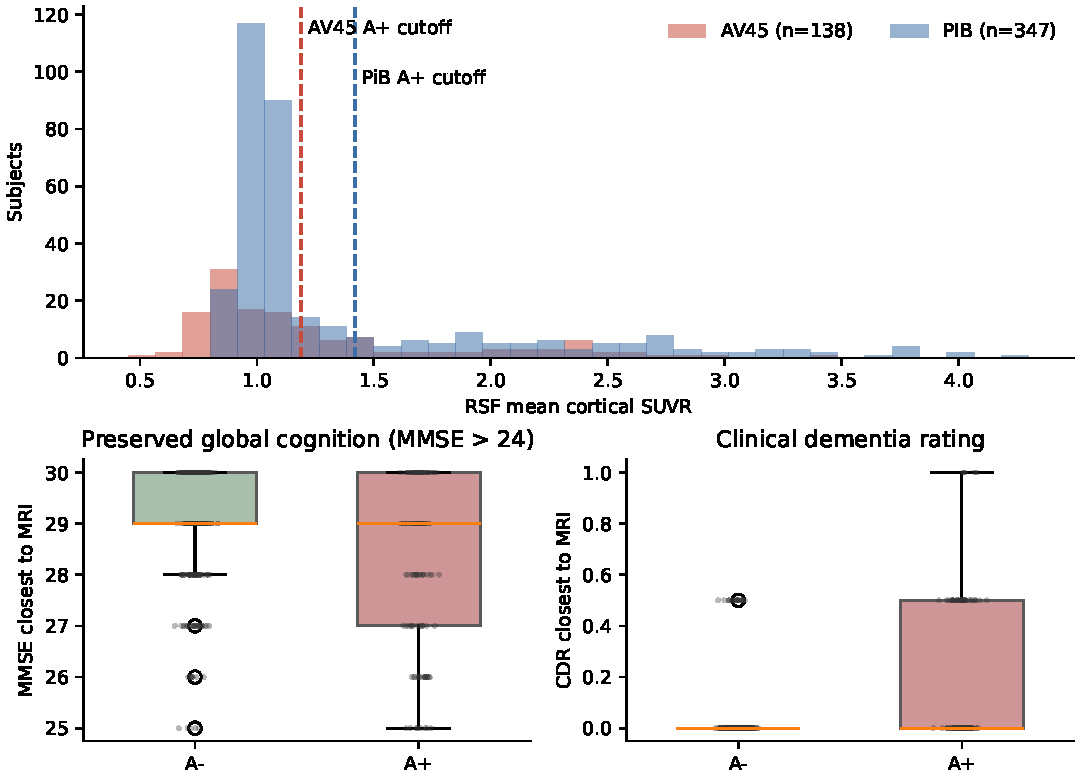
\includegraphics[width=.95\linewidth]{figs/pet_cohort_summary.pdf}
\caption{PET-linked MMSE-preserved cohort. The upper panel shows the distribution of RSF mean cortical SUVR by tracer with OASIS-3 amyloid-positivity cutoffs. Lower panels show MMSE and CDR closest to MRI for A- and A+ groups.}
\label{fig:pet_cohort}
\end{figure}

\subsection{MRI processing}

T$_1$-weighted MRI data were processed with the BrainSuite Anatomical Pipeline \cite{shattuck_brainsuite_2002}. Cortical extraction included skull stripping, bias correction, tissue classification, cortical surface modeling, and cortical thickness estimation using a partial-volume-aware anisotropic diffusion method \cite{joshi2018using}. Subject data were mapped to the USCBrain atlas using surface-constrained volumetric registration \cite{joshi_method_2012,joshi2022hybrid}. This provided a common cortical surface for group statistics.

Resting-state fMRI data were processed with the BrainSuite Functional Pipeline, which uses components from BrainSuite, FSL, and AFNI \cite{jenkinson2012fsl,cox2012afni}. Processing included motion correction, skull stripping, grand-mean scaling, temporal filtering, detrending, spatial smoothing, nuisance regression, registration to T$_1$w MRI, and mapping to USCBrain grayordinate space \cite{glasser2013minimal}. ALFF-Z was computed from the preprocessed BOLD signal using the 0.01--0.1 Hz band \cite{zuo2010oscillating}. BrainSync was used in the exploratory pairwise fMRI regression analysis \cite{joshi2018740,joshi_pairwise_2021}.

\subsection{Statistical analysis}

For PET structural analysis, pointwise cortical thickness was correlated with the closest amyloid PET RSF mean cortical SUVR in the MMSE-preserved image-quality subset. P-values were computed from Pearson correlations and corrected across the cortical surface using the Benjamini-Hochberg false discovery rate (FDR) procedure \cite{fisher1915frequency,benjamini_1995_controlling_false_discovery}. The available surface analysis used n=398 participants after image-quality filtering and did not include age or sex covariates; given the demographic imbalance reported below, this surface result is interpreted as exploratory PET-linked structural evidence.

For PET-defined resting-state motor connectivity, we used 10 motor and motor-adjacent USCBrain ROIs selected to cover superior and inferior precentral gyrus, superior and inferior postcentral gyrus, superior parietal region, parahippocampal region, and anterior/middle cingulate regions. ROI-mean time series were normalized and converted to subject-level correlation matrices. A+ and A- groups were compared edge-wise with Mann-Whitney tests, and FDR correction was applied to unique off-diagonal ROI pairs. We also fit an exploratory edge-wise linear model with amyloid status, age, and sex as predictors.

Exploratory functional analyses used MMSE as a continuous cognitive-severity variable: ALFF-Z correlation with MMSE, motor-network comparison between MMSE groups, and BrainSync pairwise regression of synchronized rs-fMRI time-series distances against MMSE differences. These analyses provide cognitive-severity context rather than a primary AD-status definition.

\section{Results}

\subsection{PET-linked cohort}

The PET-linked cohort is summarized in Table \ref{tab:cohort} and Fig. \ref{fig:pet_cohort}. A+ participants were older than A- participants (72.73$\pm$6.62 vs. 65.91$\pm$8.67 years, Welch $p=1.5\times10^{-18}$) and the sex distribution differed between groups (female/male: 64/74 in A+ vs. 206/141 in A-; $\chi^2$ $p=0.013$). A+ participants had lower MMSE despite all participants having MMSE $>24$ (28.43$\pm$1.58 vs. 29.05$\pm$1.15, Welch $p=5.1\times10^{-5}$). CDR was also higher in the A+ group (0.18$\pm$0.28 vs. 0.03$\pm$0.12, Mann-Whitney $p=2.3\times10^{-13}$); the cohort included 418 participants with CDR 0, 62 with CDR 0.5, and 5 with CDR 1. Across all PET-linked MMSE-preserved participants, amyloid SUVR was weakly but significantly associated with lower MMSE (Spearman $\rho=-0.13$, $p=0.004$).

\subsection{Amyloid PET SUVR and cortical thickness}

The available PET-based cortical-thickness analysis showed significant FDR-corrected association between amyloid PET SUVR and cortical thickness across bilateral sensorimotor cortices, cingulate cortex, parietal regions, temporal regions, precuneus, and insula (Fig. \ref{fig:pet_thickness}). The involvement of precentral and postcentral regions provides PET-linked structural evidence that motor and sensorimotor cortex may be involved in amyloid-positive adults with preserved MMSE. Because this surface map was based on unadjusted correlations and A+ participants were substantially older, the result should not be interpreted as an age-independent or AD-specific cortical-thinning effect.

\begin{figure}[t]
\centering
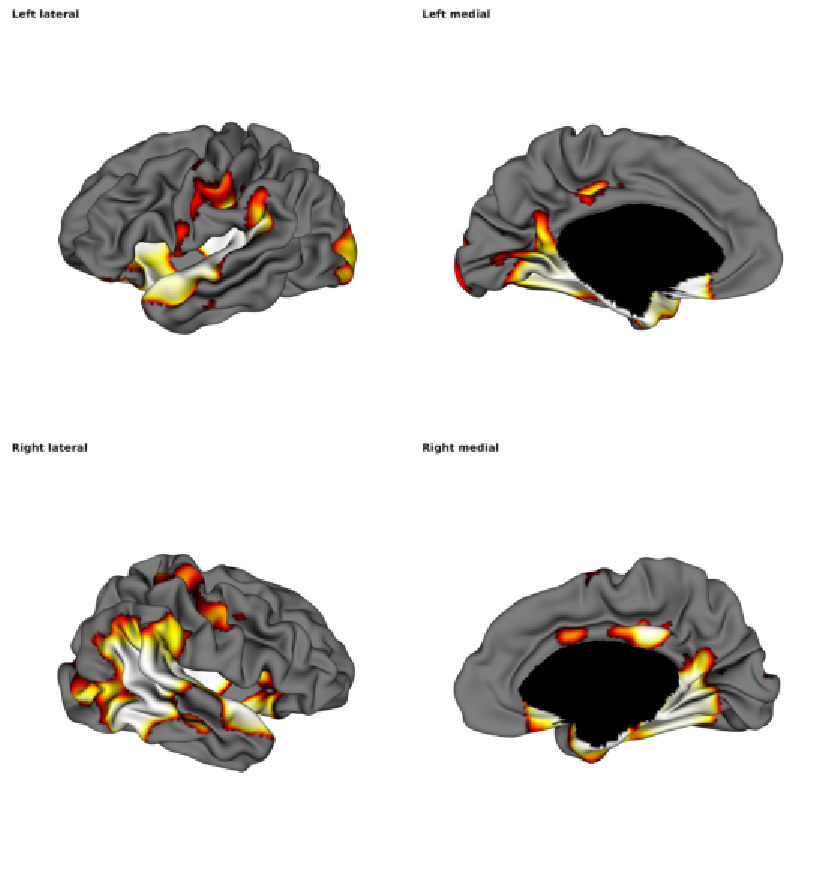
\includegraphics[width=.95\linewidth]{figs/pet_thickness_suvr_fdr.pdf}
\caption{Cortical-thickness association with amyloid PET SUVR. Maps show FDR-thresholded p-values from the available PET/SUVR cortical-thickness analysis in the MMSE-preserved image-quality subset (n=398). Significant regions include bilateral sensorimotor cortex and motor-adjacent cingulate/parietal areas. The map is exploratory because the available vertexwise analysis was not age/sex adjusted.}
\label{fig:pet_thickness}
\end{figure}

\subsection{PET-defined motor-network connectivity}

From 483 candidate rs-fMRI scans, PET-defined motor-connectivity analysis included 480 usable scans after excluding three participants with non-finite ROI time series (A-: 346; A+: 134).
 Mean connectivity matrices showed modest group differences (Fig. \ref{fig:pet_connectivity}). The strongest uncorrected edge was between left middle cingulate and inferior postcentral regions (A+ minus A- difference = 0.070, Cohen's $d=0.20$, $p=0.002$), but it did not survive FDR correction ($q=0.091$). The second strongest uncorrected edge was between parahippocampal and right middle cingulate regions ($p=0.006$, $q=0.124$). In the age/sex-adjusted edge-wise linear model, no amyloid-status term survived FDR correction; the minimum adjusted-model value was $q=0.921$, and the uncorrected cingulate-postcentral edge attenuated to $p=0.349$. Thus, PET-defined resting-state motor connectivity showed only weak evidence for group differences.

\begin{figure}[t]
\centering
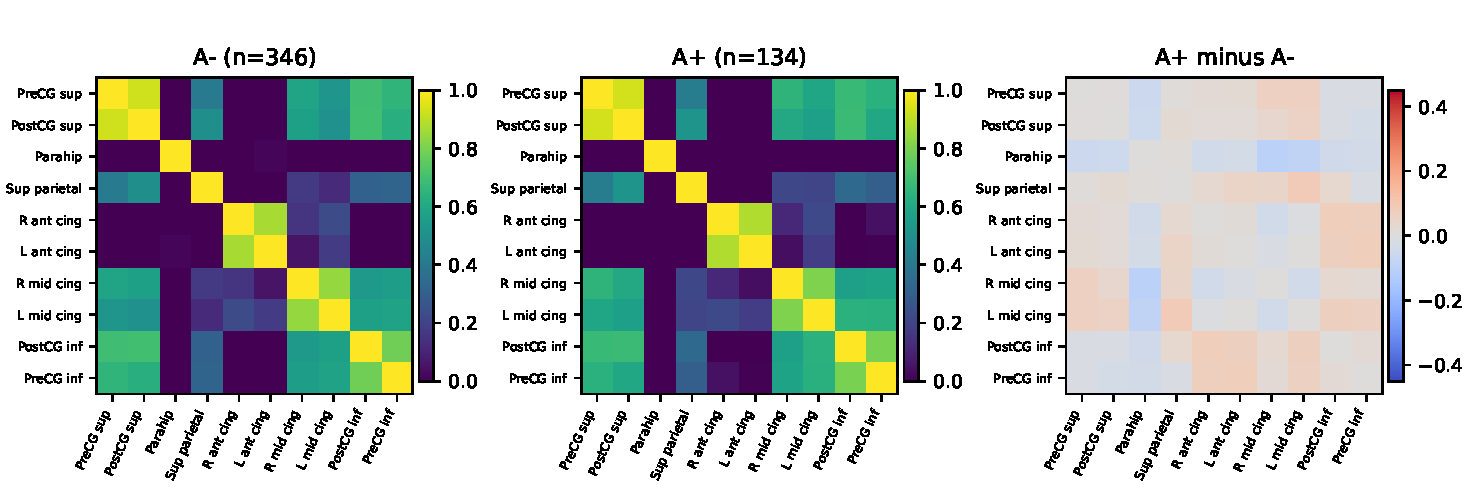
\includegraphics[width=.98\linewidth]{figs/pet_motor_connectivity.pdf}
\caption{PET-defined motor-network connectivity. A- and A+ panels show mean ROI-to-ROI resting-state connectivity. The difference panel shows A+ minus A-. No edge survived FDR correction across unique ROI pairs; the minimum unadjusted FDR value was $q=0.091$, and the minimum age/sex-adjusted edge-wise model FDR value was $q=0.921$.}
\label{fig:pet_connectivity}
\end{figure}

\subsection{Exploratory MMSE-based functional analyses}

Exploratory MMSE-based analyses provided cognitive-severity context. Grouping participants by MMSE in the preserved range produced motor-network differences in ROI analysis (Fig. \ref{fig:mmse_networks}). ALFF-Z was significantly associated with MMSE in bilateral precentral regions including the hand knob (Fig. \ref{fig:mmse_alff}). BrainSync pairwise regression also showed MMSE-related fMRI differences in bilateral motor regions and frontal/parietal cortex (Fig. \ref{fig:mmse_brainsync}). These findings are consistent with the PET-based structural result, but they should be interpreted as cognitive-severity associations rather than biomarker-defined AD status.

\begin{figure}[t]
\centering
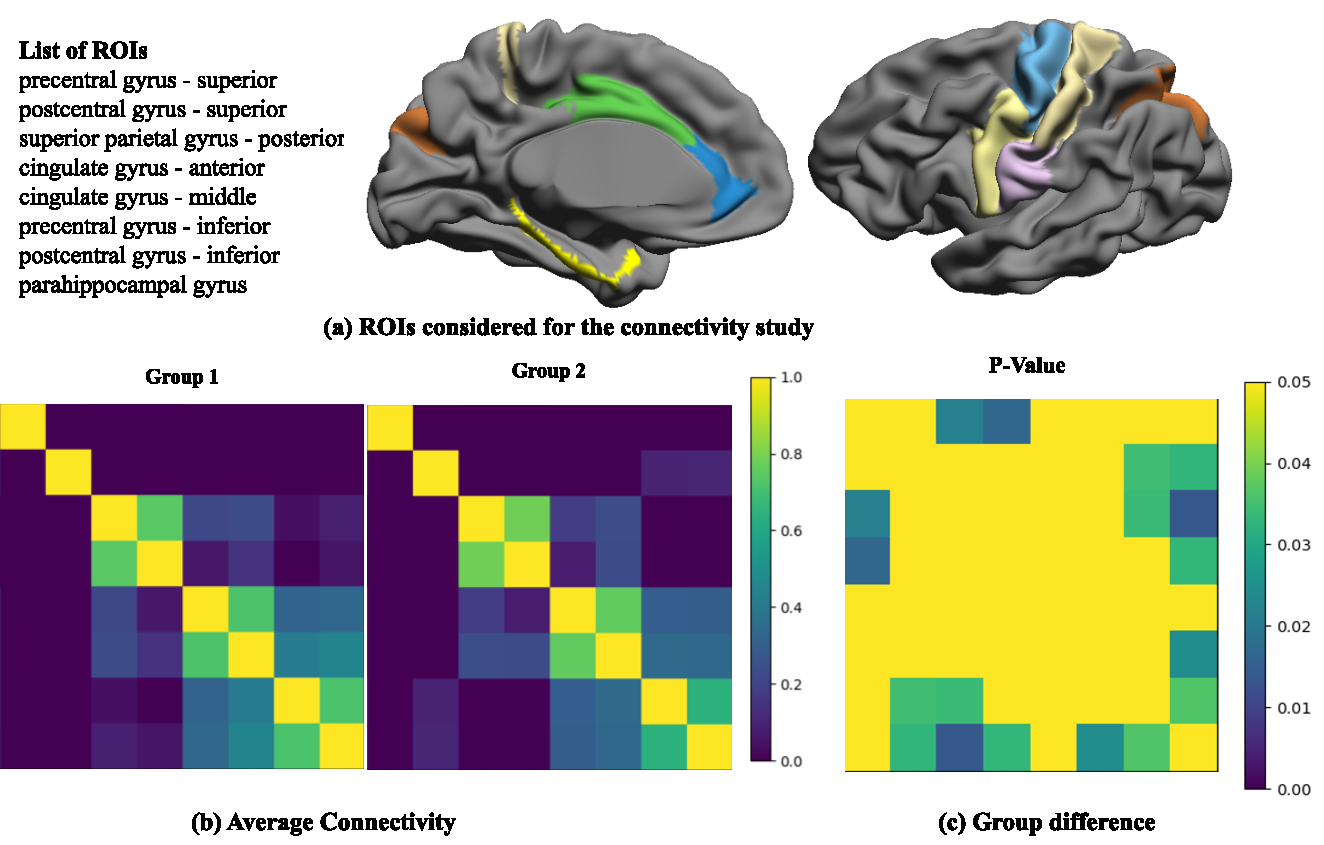
\includegraphics[width=.92\linewidth]{figs/mmse_motor_networks_v2.pdf}
\caption{Exploratory MMSE-based motor-network comparison. The grouping is based on MMSE rather than PET status and is therefore interpreted as cognitive-severity context.}
\label{fig:mmse_networks}
\end{figure}

\begin{figure}[t]
\centering
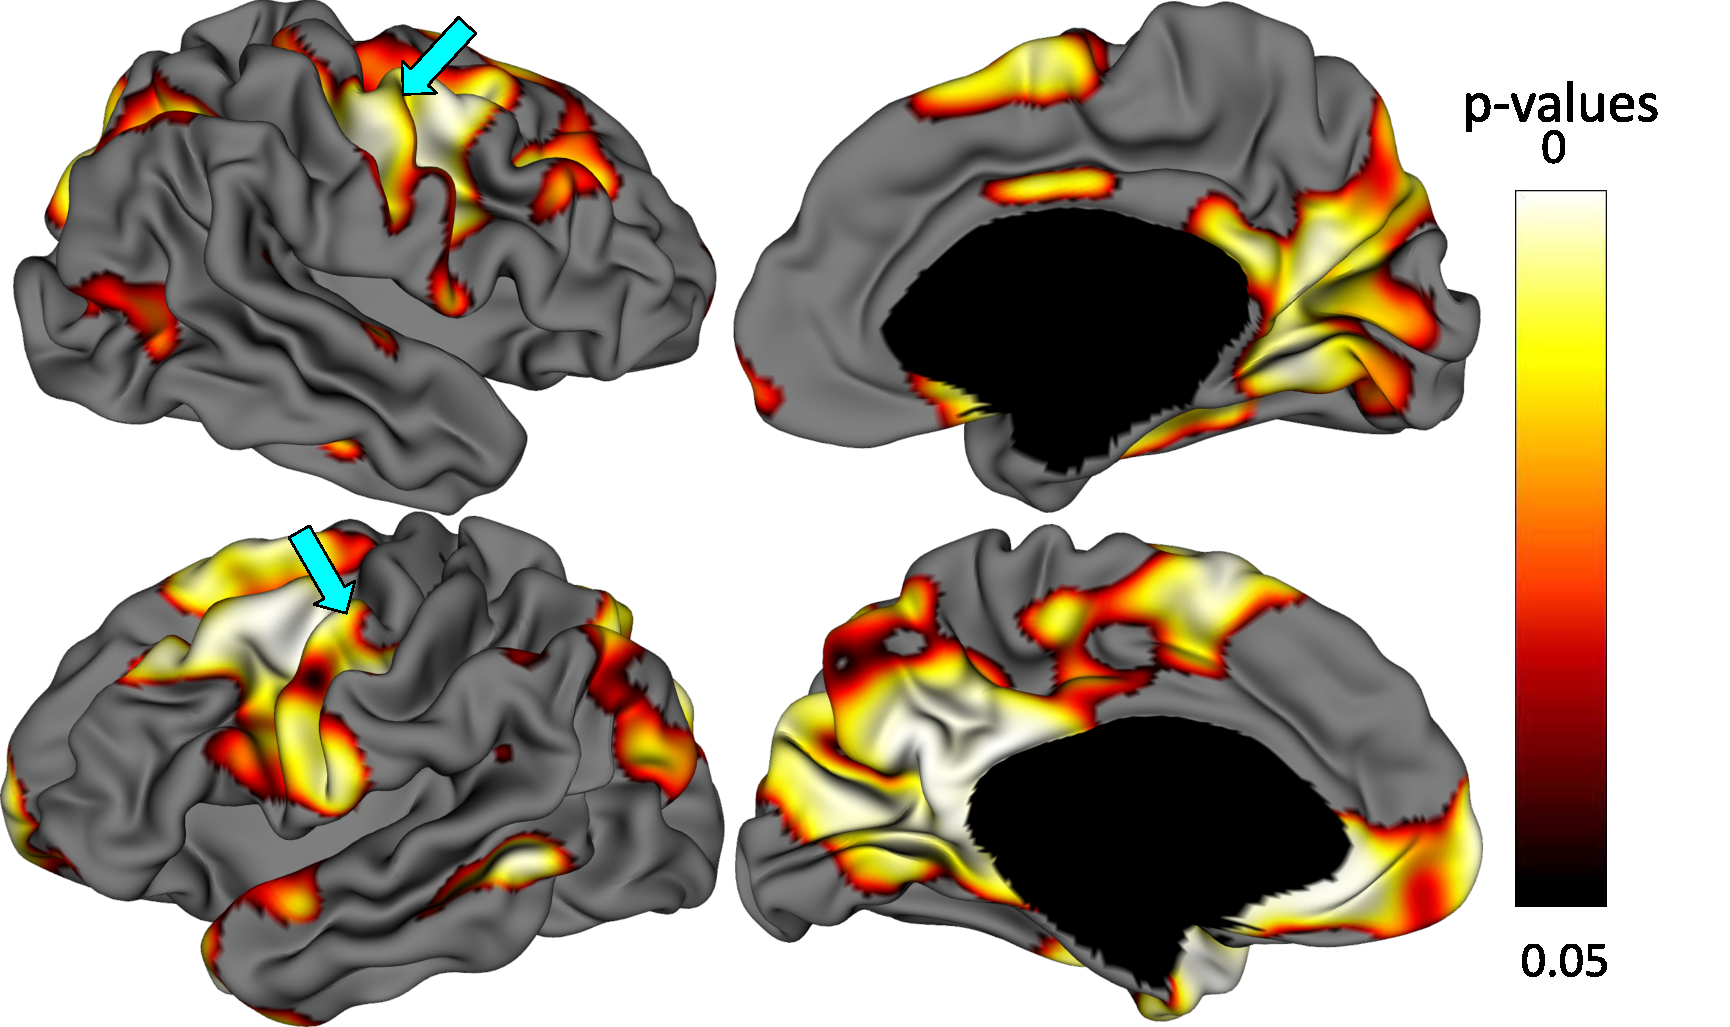
\includegraphics[width=.92\linewidth]{figs/mmse_alff_hand_knob.pdf}
\caption{Exploratory MMSE-based ALFF-Z analysis. FDR-thresholded p-values show association between MMSE and ALFF-Z in bilateral precentral regions including the hand knob.}
\label{fig:mmse_alff}
\end{figure}

\begin{figure}[t]
\centering
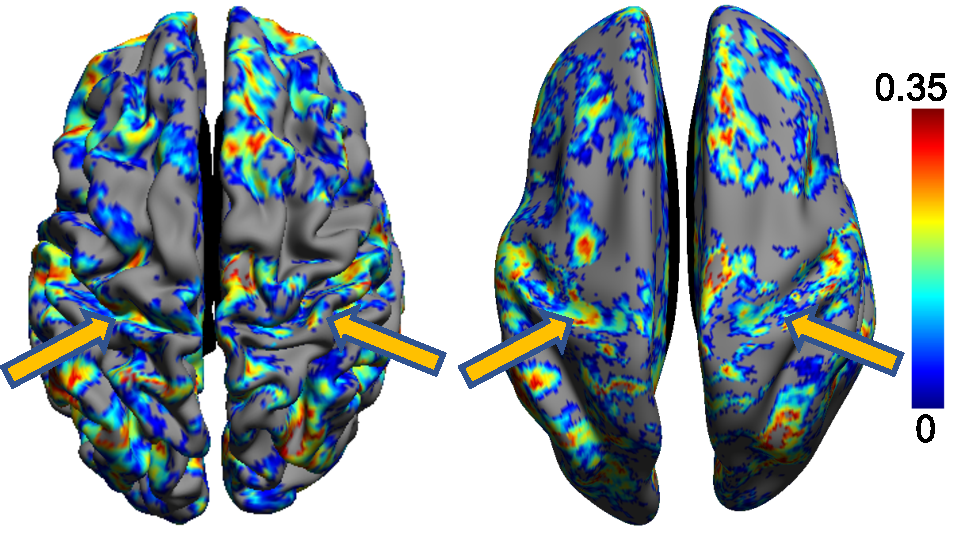
\includegraphics[width=.92\linewidth]{figs/mmse_brainsync_motor.pdf}
\caption{Exploratory MMSE-based BrainSync pairwise regression. Arrows indicate approximate hand-area motor cortex. This analysis is shown as cognitive-severity context for the primary PET-defined analyses.}
\label{fig:mmse_brainsync}
\end{figure}

\section{Discussion}

This study evaluated motor-system MRI correlates of amyloid PET burden in OASIS-3 adults with preserved MMSE. MMSE-preserved A+ adults showed a PET-linked cortical-thickness association involving sensorimotor and motor-adjacent regions. This finding suggests that motor-system structure may be related to amyloid biomarker burden, not only to cognitive screening performance. However, the interpretation must remain cautious because the A+ group was older, the sex distribution differed, and the available vertexwise surface map was not covariate adjusted.

The PET-defined resting-state motor-connectivity analysis was more modest. Several motor and motor-adjacent edges showed small uncorrected differences, especially involving cingulate and postcentral/parahippocampal regions, but none survived FDR correction, and the age/sex-adjusted edge-wise model further attenuated the apparent amyloid-status effects. This pattern is informative because resting-state fMRI may be underpowered for motor-system effects in MMSE-preserved cohorts when the relevant manual-dexterity circuits are not explicitly engaged. Task-fMRI during manual dexterity or finger-tapping paradigms may be needed to detect functional motor impairment with adequate sensitivity.

The findings fit within the AT(N) framework and contemporary biological framing of AD \cite{jack_jr_niaaa_2018,jack_revised_2024}. Amyloid PET defines A status, while cortical thickness is an MRI-based neurodegeneration measure. Published MRI/PET studies have shown that amyloid-positive clinically normal adults can have cortical thinning in AD-vulnerable regions \cite{dickerson_cortical_2009,becker_amyloid_2011}. The present results suggest that a motor/sensorimotor phenotype may also be relevant, consistent with neuropathological and biomarker studies of motor-system involvement in AD \cite{suva_primary_1999,gupta_biomarker_dexterity_2024,na_neural_basis_2025}. This does not imply that motor-cortex thinning is specific to AD, but it identifies a potentially useful motor-system phenotype for future multimodal work.

\subsection{Limitations}

First, amyloid PET provides evidence of AD pathophysiology but not tau staging, autopsy confirmation, or exclusion of non-AD copathology. Second, the cohort was selected using MMSE $>24$ rather than CDR 0 or a full neuropsychological normality definition; 67 participants had CDR 0.5 or 1. Third, A+ participants were older and differed in sex distribution. This is especially important for cortical thickness: the available PET/SUVR vertexwise map used unadjusted Pearson correlations, and the raw thickness matrices needed to regenerate a CDR 0-only or age/sex-adjusted surface map were not available in the current analysis package. Fourth, OASIS-3 was not collected as a prospective motor study, and the PET-MRI interval varied across participants. Fifth, resting-state fMRI does not directly activate manual-dexterity networks, and no behavioral dexterity measure was available for direct brain-behavior validation. Finally, the cortical-thickness maps show statistical association with continuous PET SUVR; they do not by themselves establish causal direction or individual-level classification performance.

\section{Conclusions}

Amyloid PET supports an exploratory structural association between amyloid burden and motor/sensorimotor cortex in adults with preserved MMSE. Resting-state motor connectivity differences are weak after PET-based labeling. Future studies should pair amyloid and tau biomarkers with age/sex-adjusted structural analyses, explicit manual-dexterity task-fMRI, and quantitative motor behavior. These findings support PET-linked motor-system involvement as a hypothesis requiring prospective replication.

\section*{Research in Context}

\textbf{Systematic review:} Published studies show motor slowing, impaired manual dexterity, and motor-cortex pathology in AD, but many MRI analyses use cognitive status rather than PET biomarkers to define early AD pathophysiology.

\textbf{Interpretation:} In OASIS-3 adults with MMSE $>24$, amyloid PET status and amyloid burden support exploratory structural involvement of sensorimotor cortex, with caution required because A+ participants were older and differed in sex distribution. PET-defined resting-state motor connectivity effects are weak and do not survive FDR correction.

\textbf{Future directions:} Future studies should combine amyloid and tau biomarkers with age/sex-adjusted structural analyses, task-fMRI paradigms that directly engage manual dexterity, and quantitative finger-tapping or hand-function measures.

\section*{Acknowledgements}

Data were provided by OASIS-3: Longitudinal Multimodal Neuroimaging. Principal investigators: T. Benzinger, D. Marcus, and J. Morris. OASIS-3 was supported by NIH P30 AG066444, P50 AG00561, P30 NS09857781, P01 AG026276, P01 AG003991, R01 AG043434, UL1 TR000448, and R01 EB009352.

\section*{Funding}

This work is supported by NIH grants R01EB026299, R01NS074980, R01NS121761, R01AR076088 and DoD grants W81XWH181061 and HT94252310149.

\section*{Conflict of Interest}

The authors declare no conflicts of interest relevant to this manuscript.

\section*{Data and Code Availability}

OASIS-3 data are available from the OASIS project at \url{https://sites.wustl.edu/oasisbrains/home/oasis-3/}. The analysis code and subject-level derivative tables are included with this manuscript package and will be made available at \url{https://github.com/ajoshiusc/AD_processing}. BrainSuite is open source and available from \url{https://brainsuite.org}. The BrainSuite Functional Pipeline is available from \url{https://github.com/ajoshiusc/bfp/}.

\bibliographystyle{elsarticle-num}
\bibliography{ref}

\end{document}
